\documentclass{article}

\title{Informe de Laboratorio}

%%%%%%%%%%%%%%%%%%%%%%%%%%%%%%%%%%%%%%%%%%%%%%%%%%%%%%%%%%%%%%%%%%%%%%%%%%%%
%%%%%%%%%%%%%%%%%%%%%%%%%%%%%%%%%%%%%%%%%%%%%%%%%%%%%%%%%%%%%%%%%%%%%%%%%%%%
\newcommand{\itemEmail}{vsullaq@unsa.edu.pe}
\newcommand{\itemStudent}{VLADIMIR ARTURO SULLA QUISPE}
\newcommand{\itemTeacher}{CARLO JOSE LUIS CORRALES DELGADO}
\newcommand{\itemGitHubURL}{https://github.com/Vladimir2003-debug/PW2_FINAL_PROJECT_CLIENT_MANAGER}
\newcommand{\itemCourse}{PROGRAMACION WEB 2}
\newcommand{\itemCourseCode}{20231001}
\newcommand{\itemSemester}{III}
\newcommand{\itemUniversity}{Universidad Nacional de San Agustín de Arequipa}
\newcommand{\itemFaculty}{Facultad de Ingeniería de Producción y Servicios}
\newcommand{\itemDepartment}{Departamento Académico de Ingeniería de Sistemas e Informática}
\newcommand{\itemSchool}{Escuela Profesional de Ingeniería de Sistemas}
\newcommand{\itemAcademic}{2023 - A}
\newcommand{\itemPracticeNumber}{07}
\newcommand{\itemTheme}{PROYECTO FINAL PW2 GESTION DE CLIENTES}
\newcommand{\itemInput}{10/08/2023}
\newcommand{\itemOutput}{10/08/2023}
%%%%%%%%%%%%%%%%%%%%%%%%%%%%%%%%%%%%%%%%%%%%%%%%%%%%%%%%%%%%%%%%%%%%%%%%%%%%
%%%%%%%%%%%%%%%%%%%%%%%%%%%%%%%%%%%%%%%%%%%%%%%%%%%%%%%%%%%%%%%%%%%%%%%%%%%%

% STYLE CODE
\usepackage{listings}
\usepackage{xcolor}

\definecolor{codegreen}{rgb}{0,0.6,0}
\definecolor{codegray}{rgb}{30, 82, 255}
\definecolor{codepurple}{rgb}{0.58,0,0.82}
\definecolor{backcolour}{rgb}{0.95,0.95,0.92}

\lstdefinestyle{mystyle}{
    backgroundcolor=\color{backcolour},   
    commentstyle=\color{codegreen},
    keywordstyle=\color{magenta},
    numberstyle=\tiny\color{codegray},
    stringstyle=\color{codepurple},
    basicstyle=\ttfamily\footnotesize,
    breakatwhitespace=false,         
    breaklines=true,                 
    captionpos=b,                    
    keepspaces=true,                 
    %numbers=left,                    
    numbersep=5pt,                  
    showspaces=false,                
    showstringspaces=false,
    showtabs=false,                  
    tabsize=2
}
\lstdefinestyle{ascii-tree}{
    literate={├}{|}1 {─}{--}1 {└}{+}1 
}
\lstset{style=mystyle}
\lstdefinestyle{ascii-tree}{
    literate={├}{|}1 {─}{--}1 {└}{+}1 
  }
% COLORS

%Paquetes 
\usepackage{graphicx} % Required for inserting images
\usepackage{array}
\usepackage{multirow}
\usepackage[top=3cm, bottom=3cm, outer=3cm, inner=3cm]{geometry}

\setlength{\headheight}{30pt}
\usepackage{colortbl}
\graphicspath{ {images/} }
\usepackage{listings}


\lstset{basicstyle=\ttfamily,
  showstringspaces=false,
  commentstyle=\color{red},
  keywordstyle=\color{blue}
}
\usepackage[utf8]{inputenc}
\usepackage[hidelinks]{hyperref}
\usepackage{blindtext}
\usepackage{titlesec}

\usepackage{fancyhdr}
\pagestyle{fancy}
\fancyhf{}
\setlength{\headheight}{30pt}
\renewcommand{\headrulewidth}{1pt}
\renewcommand{\footrulewidth}{1pt}
\fancyhead[L]{\raisebox{-0.2\height}{
\includegraphics[width=3cm]{img/logo_episunsa.png}}}
\fancyhead[C]{\fontsize{7}{7}\selectfont	\itemUniversity \\ \itemFaculty \\ \itemDepartment \\ \itemSchool \\ \textbf{\itemCourse}}
\fancyhead[R]{\raisebox{-0.2\height}{
\includegraphics[width=1.2cm]{img/logo_abet}}}
\fancyfoot[L]{\itemEmail }
\fancyfoot[C]{\itemCourse}
\fancyfoot[R]{Página \thepage}

% BIBLIOGRAFIA

\usepackage{biblatex} %Imports biblatex package
\addbibresource{bibliografy/references.bib} %Import the bibliography file

\begin{document}

\vspace*{30px}

\begin{center}	
		\fontsize{17}{17} \textbf{ Informe de Laboratorio \itemPracticeNumber}
\end{center}
 
\renewcommand{\arraystretch}{1.5}

\begin{tabular}{ |m{3cm}|m{2cm}|m{3cm}|m{1.2cm}|m{2.5cm}|m{1cm}| }
    \hline
    
    \multicolumn{6}{|c|}{\cellcolor{red}\textbf{INFORMACIÓN BÁSICA}} \\
    \hline
    \textbf{ASIGNATURA:} & \multicolumn{5}{|l|}{ \itemCourse} \\
    \hline
    \textbf{TITULO DE LA PRÁCTICA:} & \multicolumn{5}{|l|}{\itemTheme} \\
    \hline     
    \textbf{NÚMERO DE PRÁCTICA:} & \itemPracticeNumber & \textbf{AÑO LECTIVO:} & 2023-A & \textbf{NRO. SEMESTRE:} & \itemSemester\\
    \hline     
    \textbf{FECHA DE PRESENTACIÓN: } & \itemInput & \textbf{HORA DE PRESENTACIÓN:} & \multicolumn{3}{|l|}{ \itemOutput } \\
    \hline     
    \multicolumn{4}{|l|}{\textbf{INTEGRANTE (s):}} & & \\
    \multicolumn{4}{|l|}{- CHAISA FERNANDEZ ANTHONY LAISA}&  & \\
    \multicolumn{4}{|l|}{- MARTELL VILLANUEVA GABRIELA VANESSA}&  & \\
    \multicolumn{4}{|l|}{- SULLA QUISPE VLADIMIR ARTURO}&  & \\
    \hline
    \multicolumn{6}{|l|}{\textbf{GITHUB :} \url{\itemGitHubURL}} \\
    \hline
    \multicolumn{6}{|l|}{\textbf{URLVIDEO :} \url{https://www.youtube.com/playlist?list=PL7urz7GpHjq9A8sO27vdOfwXlYCZHMPNR}} \\
    \hline
    \multicolumn{6}{|l|}{\textbf{DOCENTE(s): }
    - \itemTeacher 
    } \\
    \hline     
\end{tabular}

\tableofcontents

\section{TIPO DE SISTEMA}

El sistema consiste en conectar Contador con sus respectivos clientes. El contador elabora catalogos de cuentas que sirven para analisis financieros. Los clientes pueden ver los catalogos y ver como estan sus estados financieros en todo momento.

\section{REQUISITOS}

El sistema debe satisfacer los siguientes requisitos funcionales y no funcionales:

\begin{itemize}
\item - RQ01 : El sistema debe estar disponible en Internet a traves de una URL.
\item - RQ02 : El sistema debe permitir el inicio/cierre de sesión.
\item - RQ03 : El sistem debe permitir a los contadores hacer las labores de CRUD
\item - RQ04 : El sistema debe evitar que los clientes puedan eliminar los catalogos y su edicion sin la autorizacion de un contador   
\item - RQ05 : El sistema debe permitir el envio de mensajes mediante su correo electronico  
\item - RQ06 : Los catalogos pueden verse y descargarse en formato pdf 
\end{itemize}

\section{MODELO DE DATOS}
El modelo de datos esta conformado por las siguientes entidades.

\begin{itemize}
\item - Usuario : La entidad principal que se ramifica en dos entidades
\item - Cliente : El cliente puede logearse y ver catalogos
\item - Contador : El contador se encarga de la elaboracion de catalogos y su manipulacion ya que tiene la autorizacion legal para hacerlo
\end{itemize}
\newpage


\section{DIAGRAMA ENTIDAD RELACION}

\begin{figure}[h]
    \centering
    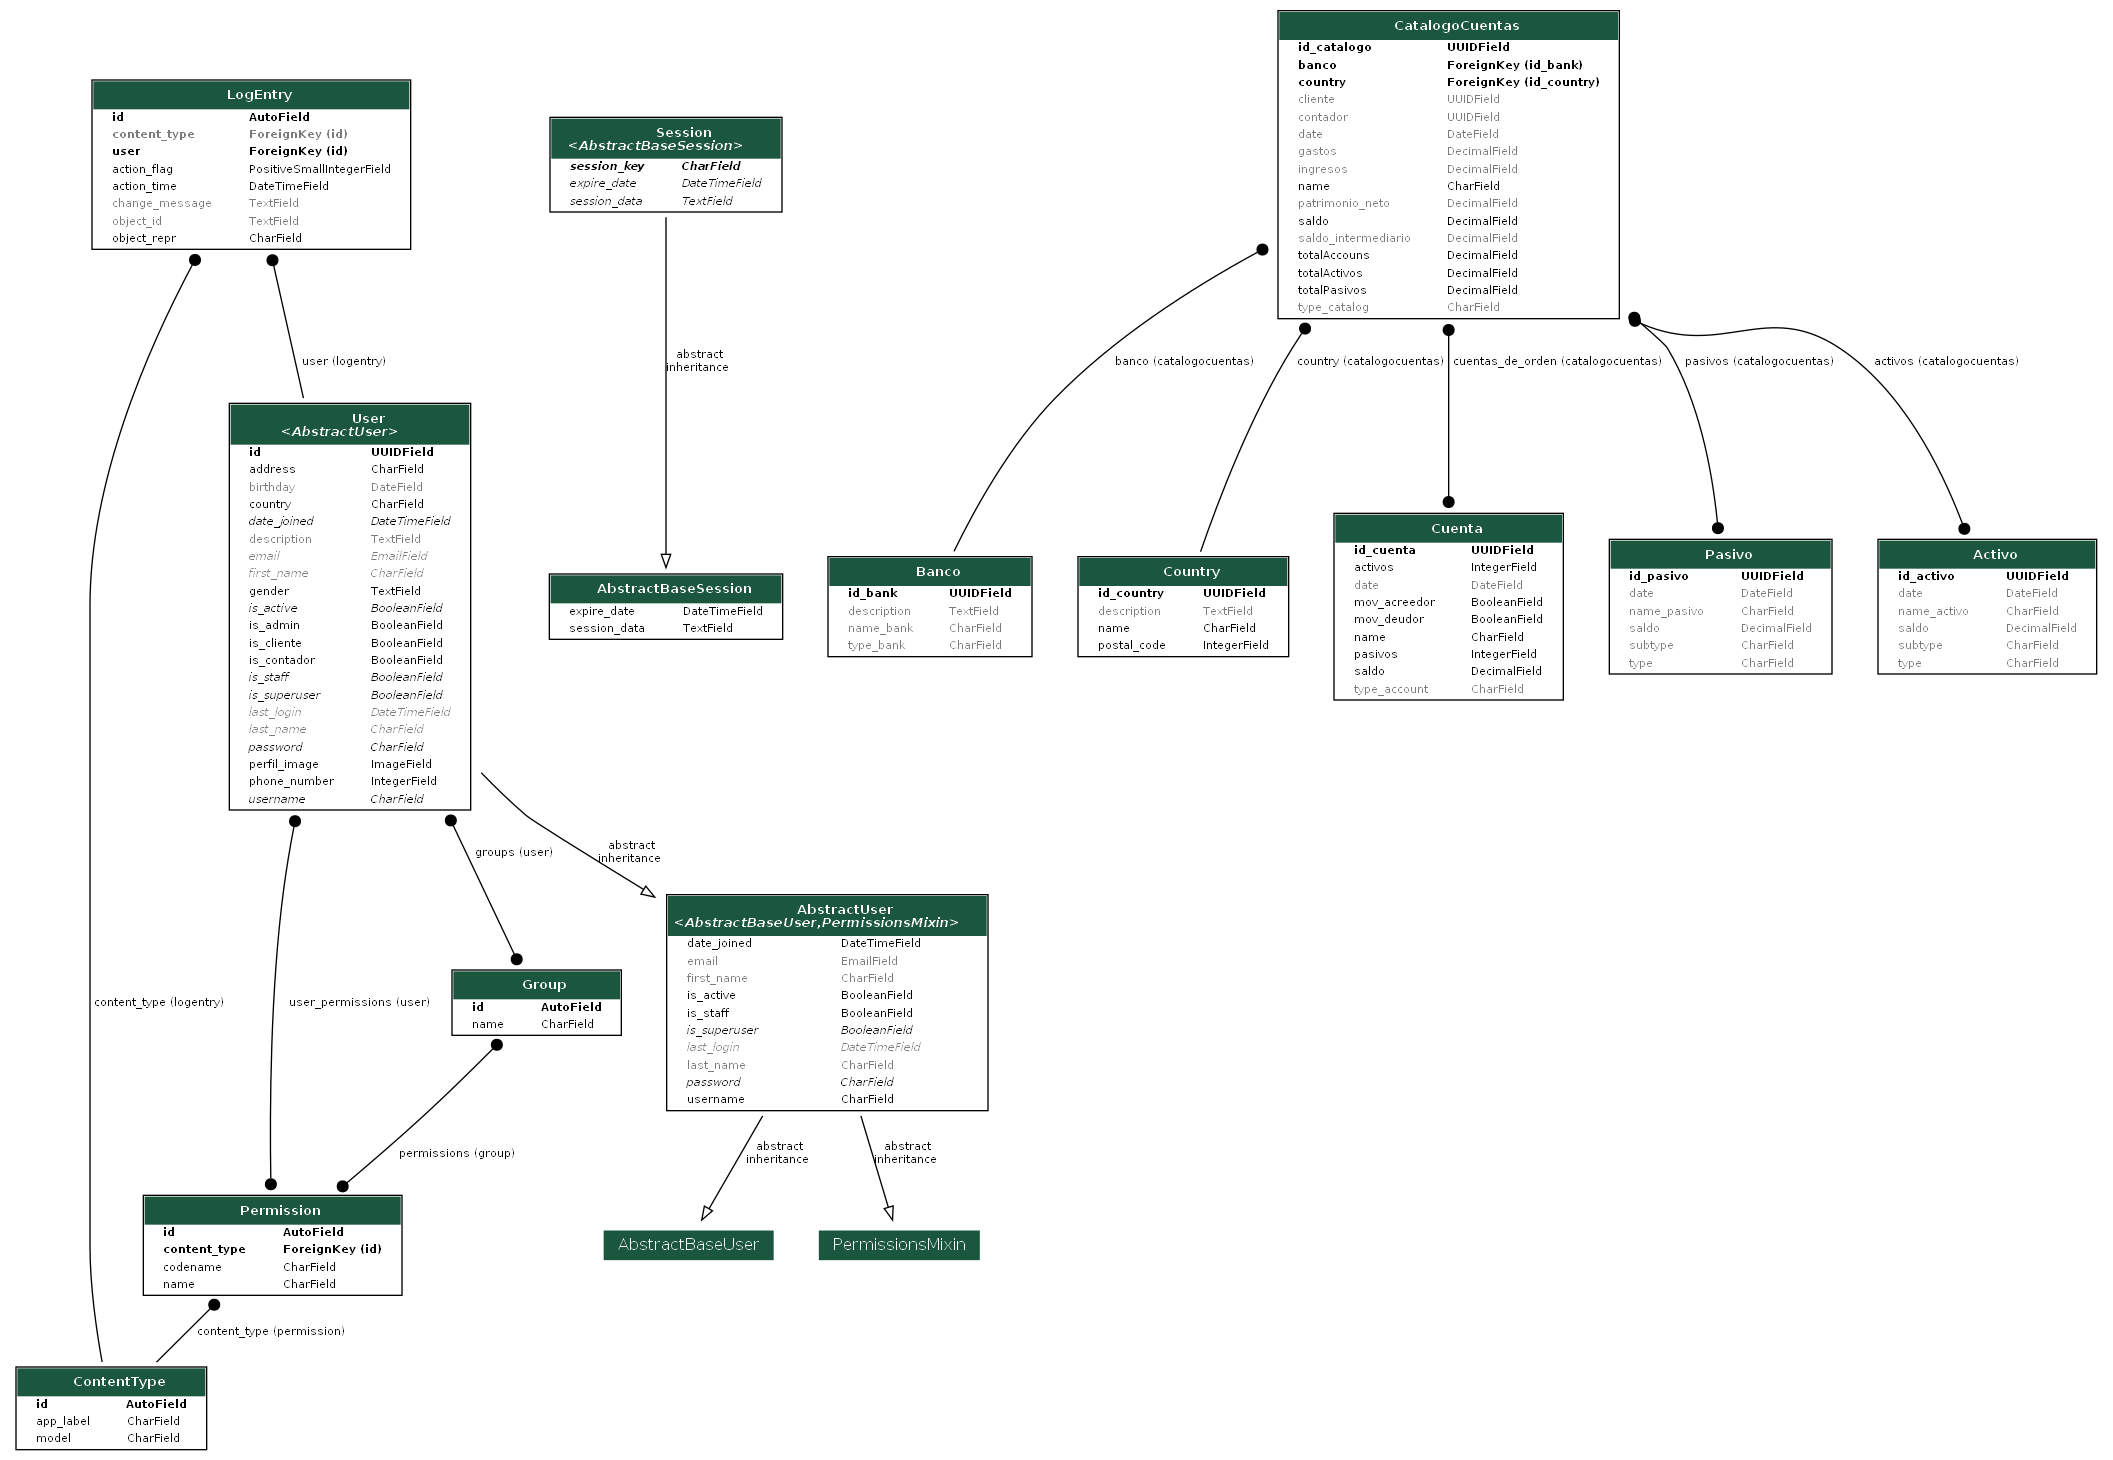
\includegraphics[scale=0.2]{img/myapp_models.png}
    \caption{diagrama entidad relacion}
    \label{fig:mesh1}
\end{figure}

\section{ADMINISTRACION DE DJANGO}
Para la creacion del proyecto consistio en lo siguiente
- Elaboraicon del modelo
- Distribucion de las apliaciones en diferentes ramas
- combinar cada apliacion con su recpectivo uso hacia otras apps
- Usar templates en el proyecto para hacerlo mas vistoso

Problemas durante el desarrollo
- imposibilidad de usar ajax
- problemas con bases de datos (especialmente windows)
- retiro de uno de los compañeros 


\section{CRUD - Core Business - Clientes finales}
El núcleo de negocio del sistema de inscripciones tiene valor de aceptación para los cliente finales (alumnos) radica en realizar el proceso de inscripción propiamente, que empieza desde que:
1. Tanto el Cliente como el Contador pueden iniciar sesion
2. El contador puede crear y elaborar catalogos el cliente solo puede mirar.
3. Los catalogos se pueden ver y descargar en formato pdf .
4. Los ususarios pueden enviar mensajes
6. El usuario puede cerrar sesion.

Todas y cada una de estas pantallas debe funcionar en la plantilla bootstrap.
A continuación se muestran las actividades realizadas para su construcción:


\section{Servicios mediante una API RESTful}
Se ha creado una aplicación que pondra a disposición cierta información para ser consumida por otros clientes HTTP.
1. GET : Con el método get se devolverá la lista de activos,pasivos y catalogos y horarios establecidos En formato JSON.

\section{TEMPLATES}

https://www.bootdey.com/snippets/view/profile-edit-data-and-skills

\section{Investigación: Email, Upload.}
- Email: Se utilizará la funcionalidad del uso de envío de correos electrónicos cuando el proceso de inscripciones culmine y al profesor le llegue la lista de alumnos inscritos en sus grupos a cargo.
- Render PDF: Se utilizará esta funcionalidad para renderizar y elaborar pdfs 

\section{DICCIONARIO DE DATOS}

\begin{table}[H]
    \centering
    \begin{tabular}{|c|c|c|c|c|c|}
    \hline
Use	& & & & & \\		
\hline
Atributo &	Tipo &	Nulo &	Clave &	Predeterminado &	Descripción \\
\hline
id &	UUID	& No &	Si	& uuid.UUID &	Código\\
\hline
name	&Cadena	&No	&No&	Ninguno	&Nombre \\
\hline
first_name&	Cadena&	No&	No	&Ninguno&	Primer Nombre \\
\hline
last_name&	Cadena&	No&	No&	Ninguno&	Apellido\\
\hline
is_admin&	Boolean&	No&	No	&Ninguno&	Confirmacion para ver si es administrador \\
\hline
is_cliente&	Boolean	&No	&No&	Ninguno	&Verificacion de entidad cliente \\
\hline
is_contador&	Boolean&	No&	No	&Ninguno	&verificacion de entidad coontador \\
\hline
    \end{tabular}
    \caption{USER}
    \label{}
\end{table}

\begin{table}[H]
    \centering
    \begin{tabular}{|c|c|c|c|c|c|}
    \hline
Banco	& & & & & \\		
\hline
Atributo&	Tipo&	Nulo&	Clave&	Predeterminado&	Descripción\\
\hline

id_bank&	UUID&	No&	Si&	uuid.UUID&	Código\\
\hline

name_bank&	Cadena&	No&	Si	&Ninguno	&nombre\\
\hline

type_bank	&Cadena&	No	&No	&Ninguno&	tipo\\
\hline

description&	Cadena	&No	&No&	Ninguno&	que tiene que decir del banco\\
\hline
    \end{tabular}
    \caption{BANCO}
    \label{}
\end{table}

\begin{table}[H]
    \centering
    \begin{tabular}{|c|c|c|c|c|c|}
    \hline
Country	& & & & & \\	
\hline

Atributo	&Tipo&	Nulo&	Clave&	Predeterminado&	Descripción\\
\hline

id_country&	UUID&	No	&Si	&uuid.UUID	&Código\\
\hline

name&	Cadena&	No&	No&	Ninguno&	nombre\\
\hline

description	&Cadena&	No	&No	&Ninguno	&descripcion\\
\hline

postal_code	&decimal	&No	&No	&Ninguno	&codigo postal del pais\\
\hline
    \end{tabular}
    \caption{COUNTRY}
    \label{}
\end{table}


\begin{table}[H]
    \centering
    \begin{tabular}{|c|c|c|c|c|c|}
    \hline
Activo	& & & & & \\					
\hline

Atributo	&Tipo&	Nulo&	Clave	&Predeterminado	&Descripción\\
\hline

id_activo&	UUID&	No&	Si	&uuid.UUID	&Código\\
\hline

date&	fecha	&No&	No	&Ninguno	&fecha creacion\\
\hline

type	&cadena	&No	&No&	Ninguno&	typo del activo\\
\hline

subtype	&cadena&	No&	Si&	Ninguno&	sub tipo del activo\\
\hline
name_activo&	Cadena&	No&	Si&Ninguno	nombre\\
\hline

saldo&	decimal&	No	&No	&Ninguno&	saldo\\
\hline
    \end{tabular}
    \caption{ACTIVO}
    \label{}
\end{table}

\begin{table}[H]
    \centering
    \begin{tabular}{|c|c|c|c|c|c|}
    \hline
pasivo	& & & & & \\	
\hline

Atributo&	Tipo&	Nulo&	Clave&	Predeterminado	&Descripción\\
\hline

id_pasivo&	UUID&	No&	Si&	uuid.UUID&	Código\\
\hline

date&	fecha&	No	&No	&fecha actual&	fecha creacion\\
\hline

type&	cadena	&No	&No&	Ninguno	&typo del activo\\
\hline

subtype&	cadena&	No&	Si&	uuid.UUID&	sub tipo del pasivo\\
\hline

name_pasivo&	Cadena&	No	&Si	&Ninguno	&nombre\\
\hline

saldo&	decimal&	No	&No	&Ninguno	&saldo\\
\hline
    \end{tabular}
    \caption{PASIVO}
    \label{}
\end{table}


\begin{table}[H]
    \centering
    \begin{tabular}{|c|c|c|c|c|c|}
    \hline
Cuenta	& & & & & \\				
\hline

Atributo&	Tipo	&Nulo&	Clave&	Predeterminado	&Descripción\\
\hline

id_cuenta&	UUID&	No&	Si	&uuid.UUID	&Código\\
\hline

type_accountr&	Cadena&	No&	Si	&Ninguno	&el tipo de la cuenta\\
\hline

name	&Cadena&	No&	No&	Ninguno&	nombre\\
\hline

date	&fehca	&No	&No&	Ninguno&	fecha de creacion\\
\hline

activos	&Cadena&	No	&No&	Ninguno	&haber\\
\hline

pasivos	&Cadena&	No	&No	&Ninguno	&debe\\
\hline

saldos	&Cadena&	No&	No&	Ninguno	&saldo\\
\hline

mov_deudor&	Boolena	&No	&No	&Ninguno	&si el cliente tiene deuda\\
\hline

mov_acreedor&	Boolean&	No&	No	&Ninguno&	si el cliente excede su cuente\\
\hline
    \end{tabular}
    \caption{CUENTA}
    \label{}
\end{table}

\begin{table}[H]
    \centering
    \begin{tabular}{|c|c|c|c|c|c|}
    \hline
CatalogoCuentas	& & & & & \\				
\hline

Atributo&	Tipo&	Nulo&	Clave&	Predeterminado&	Descripción\\
\hline

id_catalogo&	UUID	&No&	No	&uuid.UUID	&Código\\
\hline

country	&Cadena	&No	&No	&Ninguno	&pais del catalogo\\
\hline

date&	Cadena&	No	&No	&fecha actual	&fecha\\
\hline

type_catalog&	cadena&	No	&No&	Ninguno	&tipo del catalogo\\
\hline

banco&	cadena&	No	&No	&Ninguno&	Código\\
\hline

name	&cadena	&No	&No&	Ninguno	&Código\\
\hline

activos&	activo	&No	No&	Ninguno&	Código\\
\hline

pasivos	&pasivo&	No	&No&	Ninguno	&Código\\
\hline

patrimonio_neto	&decimal&	No&	Si	&Ninguno&	nombre\\
\hline

gastos	&decimal	&No	&No&	Ninguno&	tipo\\
\hline

ingresos	&decimal	&No	&No&Ninguno&	nombre\\
\hline

saldos_intermedios&	decimal&	No	&No	&Ninguno&	tipo\\
\hline

cuentas_de_orden&	cuenta	&No	&No&	Ninguno	&nombre\\
\hline

cliente&	uuid	&No	&No&	Ninguno&	tipo\\
\hline

contador&	uuid&	No&	No&	Ninguno	&nombre\\
\hline

totalActivos&	decimal&	No	&No&	Ninguno	&tipo\\
\hline

totalPasivos	&decimal&	No&	Si&	Ninguno&	nombre\\
\hline

totalAccounts	&decimal	&No&	No	&Ninguno	&tipo\\
\hline
    \end{tabular}
    \caption{CATALOGO DE CUENTAS}
    \label{}
\end{table}

\printbibliography[
heading=bibintoc,
title={References}
]

\end{document}
